\documentclass{academic-template}

\usepackage{graphicx}
\usepackage{booktabs}
\usepackage{pgfplots}
\pgfplotsset{compat=1.18}
\usepackage{hyperref}

\title{Creating PDF Documents Using LaTeX}
\author{Mohamad Masarwa}
\date{\today}

\begin{document}

\maketitle

\begin{abstract}
LaTeX is one of the most widely used document preparation systems in academia, engineering, computer science, and scientific publishing. This report presents the principles of creating professional PDF documents using LaTeX and LuaLaTeX. The document demonstrates text formatting, document organization, tables, figures, graphs, references, and bibliography management. In addition, it evaluates the advantages and limitations of LaTeX compared to traditional word-processing software and discusses its role in modern academic publishing.
\end{abstract}

\tableofcontents

\newpage

\section{Introduction}

Digital documents have become the standard medium for academic communication. Researchers, students, engineers, scientists, and educators produce reports, articles, books, and technical documentation every day. While traditional word processors provide a convenient visual editing environment, many academic institutions and publishers prefer documents created using LaTeX because of their consistency, flexibility, and professional appearance.

LaTeX allows authors to focus on content rather than formatting. The system automatically manages document structure, numbering, references, tables, figures, and bibliographies. This approach enables the creation of highly organized and visually appealing documents.

\section{History of TeX and LaTeX}

The origins of LaTeX can be traced back to the development of TeX by Donald Knuth in the late 1970s. Knuth created TeX after becoming dissatisfied with the quality of typesetting available for his publications.

In the 1980s, Leslie Lamport introduced LaTeX as a set of macros built on top of TeX. These macros simplified document creation by allowing users to focus on logical structure rather than low-level formatting commands.

Today, LaTeX is widely used in universities, research institutions, and scientific journals around the world.

\section{What is LaTeX?}

LaTeX is a document preparation system based on markup commands. Instead of manually formatting text, authors describe the logical structure of a document.

The LaTeX workflow generally consists of three stages:

\begin{enumerate}
\item Writing the source code.
\item Compiling the source using a LaTeX engine.
\item Producing a PDF document.
\end{enumerate}

This workflow enables consistent and professional document production.

\section{Advantages of LaTeX}

LaTeX offers numerous advantages for academic and technical writing.

\begin{itemize}
\item Professional document layout
\item Automatic numbering of sections, figures, and tables
\item Bibliography management
\item Cross-referencing capabilities
\item Excellent mathematical typesetting
\item Platform independence
\item High-quality PDF generation
\end{itemize}

These features make LaTeX the preferred choice for researchers and engineers worldwide.

\section{Comparison Between LaTeX and Microsoft Word}

Table 1 presents a comparison between LaTeX and Microsoft Word.

\begin{table}[h]
\centering
\caption{Comparison of LaTeX and Microsoft Word}
\begin{tabular}{|l|c|c|}
\hline
Feature & LaTeX & Word \\
\hline
Professional Typesetting & Yes & Limited \\
Mathematical Support & Excellent & Moderate \\
Bibliography Management & Automatic & Semi-Automatic \\
Learning Curve & High & Low \\
Academic Publishing & Preferred & Less Common \\
\hline
\end{tabular}
\end{table}

\section{LaTeX Usage in Academic Fields}

Figure 1 illustrates the estimated popularity of LaTeX in different academic disciplines.

\begin{figure}[h]
\centering
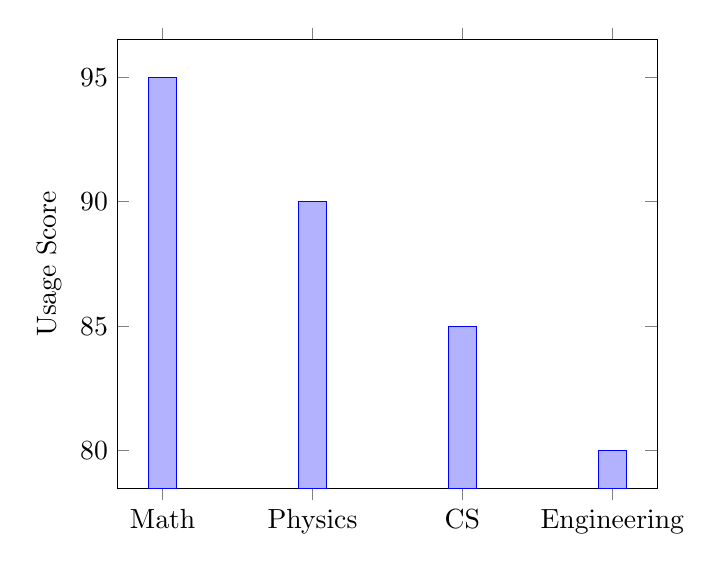
\begin{tikzpicture}
\begin{axis}[
ybar,
ylabel={Usage Score},
symbolic x coords={Math,Physics,CS,Engineering},
xtick=data
]

\addplot coordinates {
(Math,95)
(Physics,90)
(CS,85)
(Engineering,80)
};

\end{axis}
\end{tikzpicture}
\caption{Estimated popularity of LaTeX across disciplines}
\end{figure}

\section{Document Structure}

A typical LaTeX document contains three major components:

\begin{itemize}
\item Document class
\item Preamble
\item Document content
\end{itemize}

The document class determines the overall formatting rules. The preamble contains package declarations and configuration settings. The document body contains the actual content.

\section{Example Figure}

Figure 2 presents the official LaTeX Project logo.

\begin{figure}[h]
\centering

\includegraphics[width=0.55\textwidth]{latex-logo.png}
\caption{Official LaTeX Project Logo}
\end{figure}

\section{Conclusion}

LaTeX remains one of the most powerful document preparation systems available today. Its ability to manage complex documents, automate formatting tasks, and generate professional PDF outputs makes it highly valuable in academia and industry.

Although the learning curve may initially appear challenging, the long-term benefits significantly outweigh the initial effort required to master the system. As academic publishing continues to evolve, LaTeX is expected to remain a dominant tool for professional document preparation.

\section{References}

\begin{enumerate}
\item D. E. Knuth, \textit{The TeXbook}. Addison-Wesley, 1984.

\item L. Lamport, \textit{LaTeX: A Document Preparation System}. Addison-Wesley, 1994.

\item The LaTeX Project Team, ``LaTeX Project,'' Available: \url{https://www.latex-project.org}

\item Overleaf Documentation, ``Learn LaTeX,'' Available: \url{https://www.overleaf.com}
\end{enumerate}

\end{document}